\subsection{System's degrees of freedom}

CALIS is capable of deploying sources at various positions inside \lsv. Besides movement along Z up to maximum cable length, it is possible to articulate at an angle of $\theta$ between 0$^{\circ}$ and 90$^{\circ}$, where $\theta$ is the zenith-angle (Fig.~\ref{fig:coordinate_system}). Angles of more than 90$^{\circ}$ are excluded because articulation chain's end is reached at a 90$^{\circ}$ angle (see Fig.~\ref{fig:sourceArmRotation}).

\begin{figure}[htbp]
 \centering
  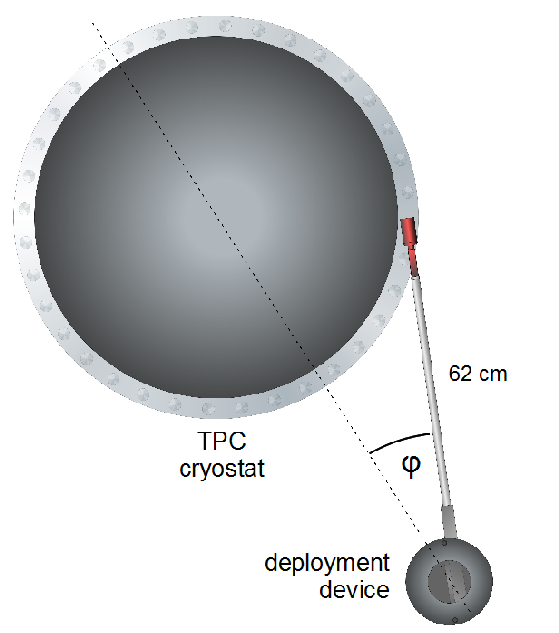
\includegraphics[height=0.37\textheight,clip=true]{Figures/DeploymentDevice_XY_view}
  \includegraphics[height=0.37\textheight]{Figures/CALIS_sideview_Cary.jpg}
  \caption{Two degrees of freedom in source deployment position after a certain source arm length has been chosen: \textit{left}: rotation in XY-plane, \textit{right:} articulation to an angle $\theta$ between 90$^{\circ}$ when arm is articulated, and at 0$^{\circ}$ when dearticulated. }
  \label{fig:coordinate_system}
\end{figure} 
%https://en.wikibooks.org/wiki/LaTeX/Importing_Graphics on clip=true removes white space around the picture - neat!

\subsubsection{XY-plane rotation}\label{sec:XYrotation}
A sealed connection below view port has an o-ring seal and uses a ring clamp to compress seal. This clamp can be slightly loosened allowing upper assembly (above and including view port) to be rotated with respect to lower assembly and detector. Rotation in XY-plane can even be performed while device is deployed next to cryostat, since seal is helium leak and light tight even when loosened.

In principle a rotation in 360$^\circ$ can be done, except when arm would interfere with cryostat. This has been used in one calibration campaign to deploy a neutron source directly next to the cryostat and rotated away by 90$^\circ$ to study optical shadowing effects from cryostat (Sec.~\ref{sec:CalibCampaigns}). 



%For articulation, there is currently a choice of three arm lengths---40.3\,cm,  57.15\,cm and 62\,cm.  
%Each of these lengths are measured from the center line of the organ pipe to the end of the source holder.  The arm lengths, 57.15\,cm and 62\,cm are intentionally made too long as they will be used to determine the exact location of the cryostat; some uncertainty in the cryostat's z and lateral position exist at the level of 3 - 4\,cm. The organ pipe we intend to use is 81\,cm distant from the cryostat center (and the geometric center of the LSV sphere) as measured from the center line of the organ pipe. The cryostat is 32\,cm in radius, which leaves a distance of $\sim$49\,cm to be reached  by the arm.


\begin{figure}[htbp]
 \centering
  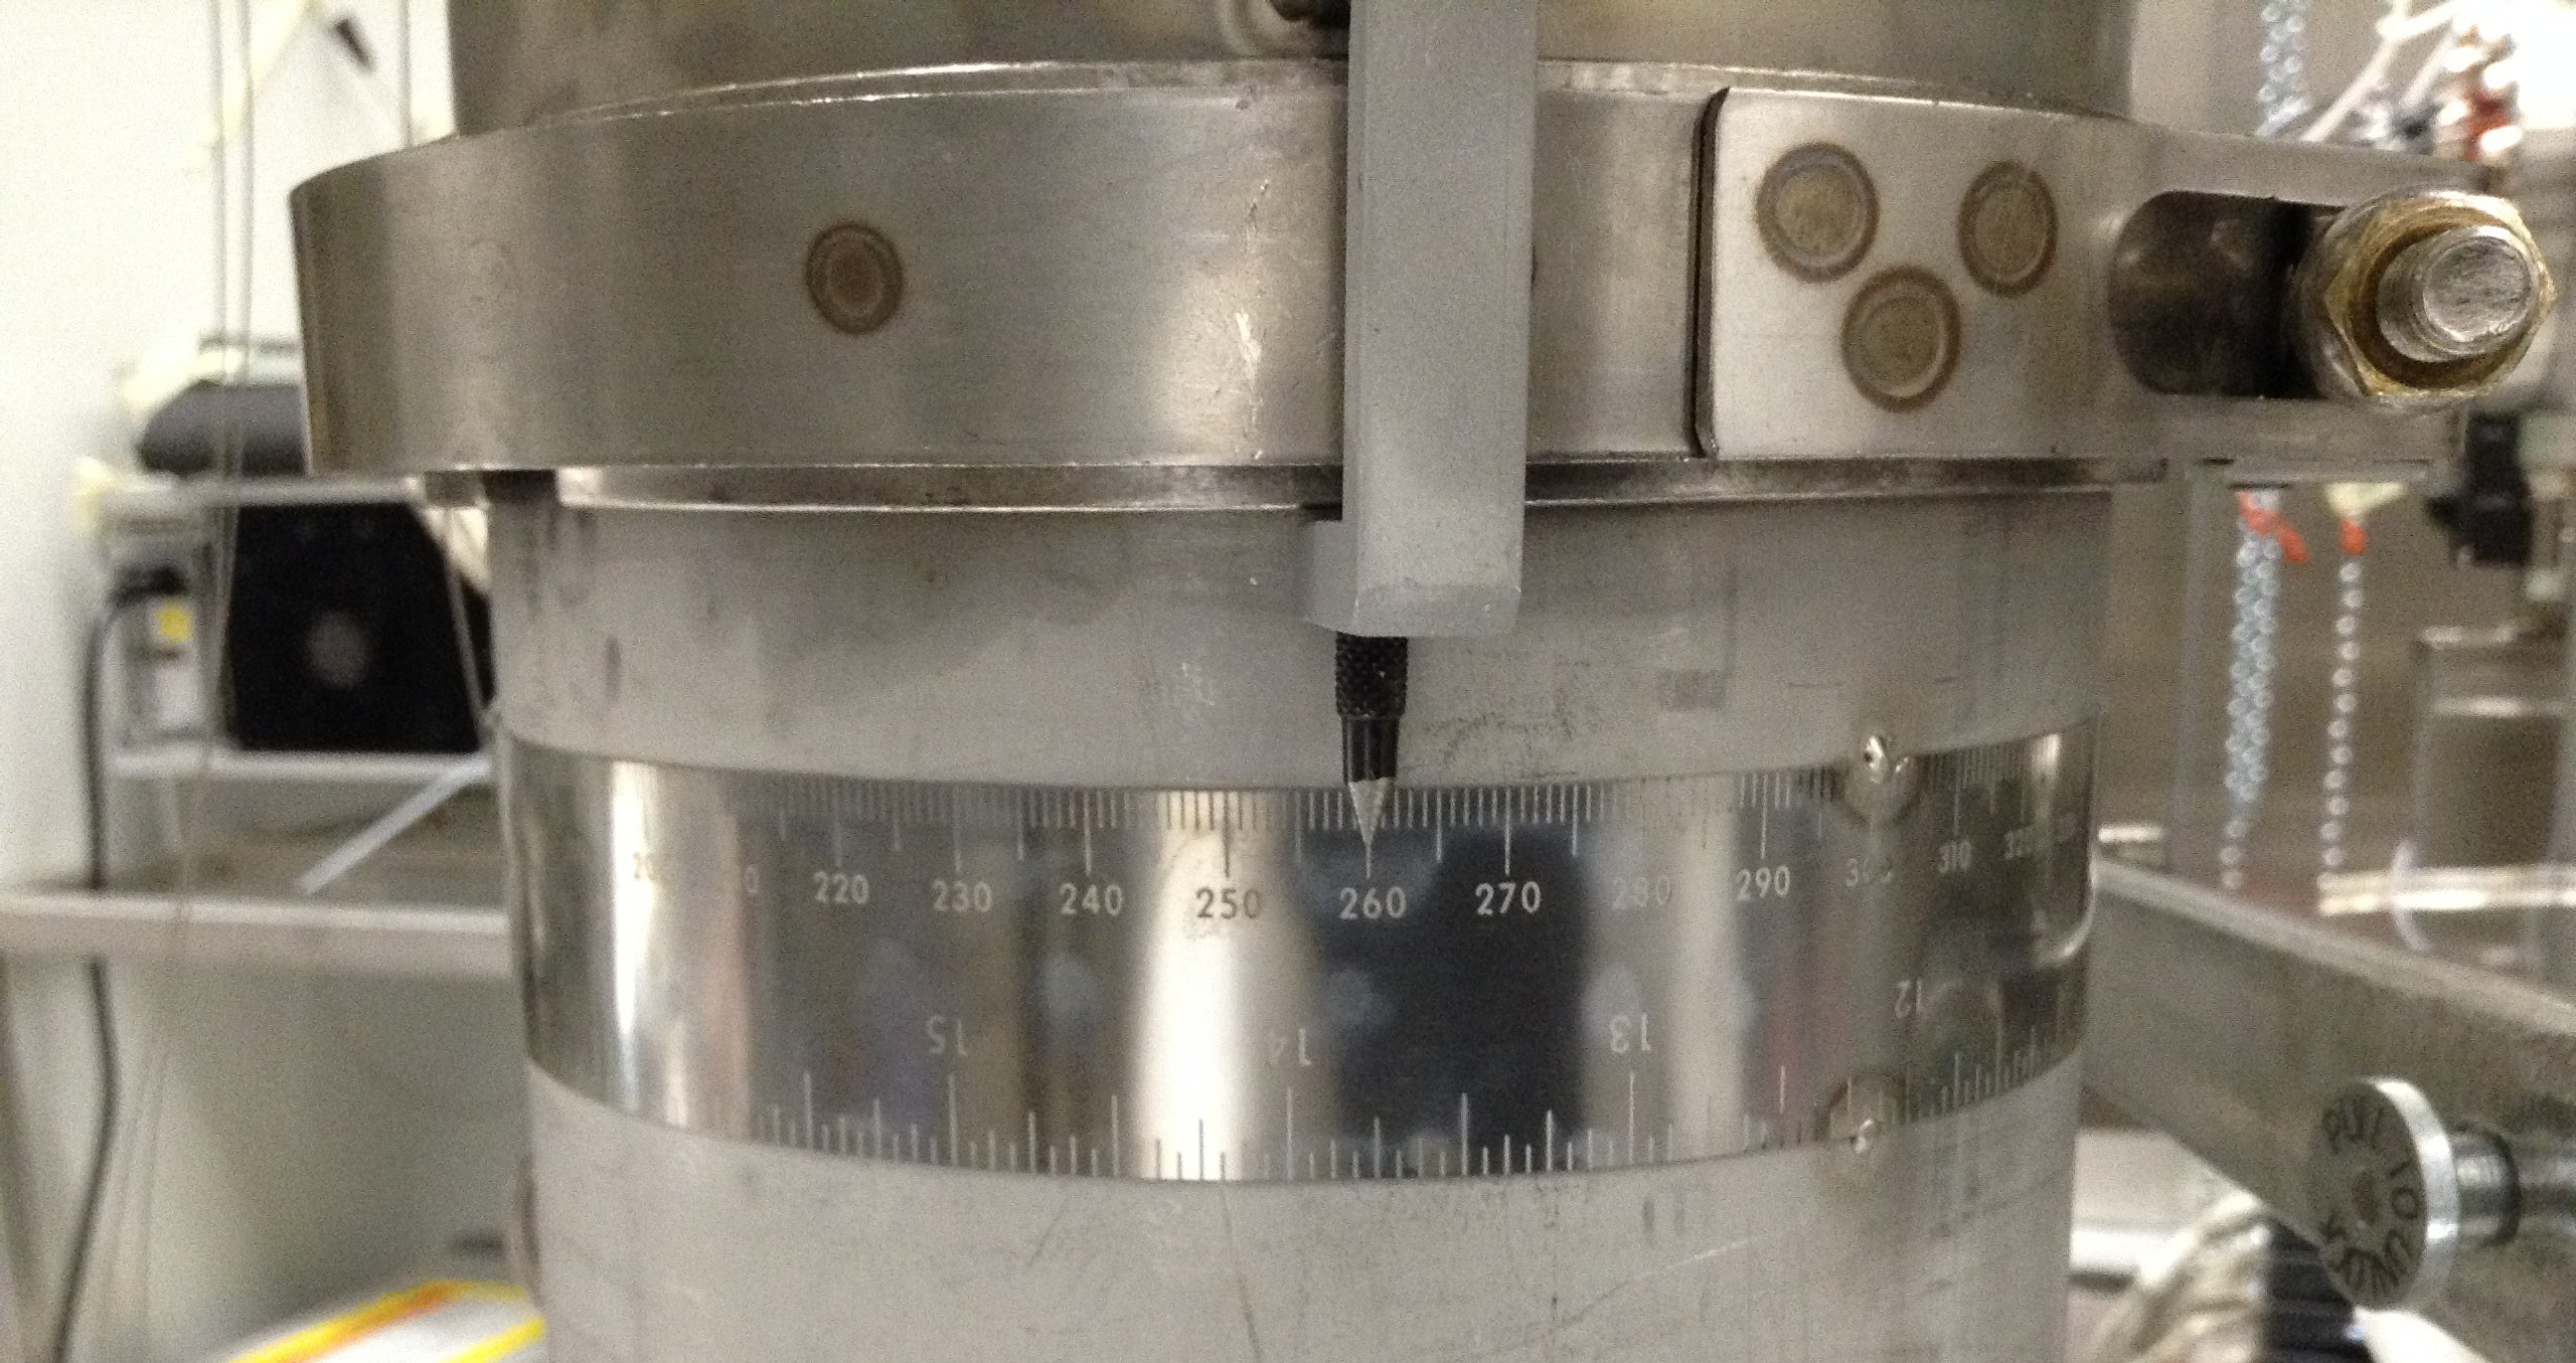
\includegraphics[width=0.7\textwidth]{Figures/RingClamp_WithPin_IMG_2669.JPG}
%  \includegraphics[scale=0.5]{Figures/RingClamp.jpg}
  \caption{Beneath view port is a ring clamp with angle measuring strip underneath. To perform azimuthal rotation, ring clamp is slightly loosened, and entire upper assembly is rotated with respect to lower assembly, along with deployment device. Rotation angle is read from strip going around the pipe. Strip is in mm, which has then been calibrated in degrees.}
  \label{fig:ring_clamp}
\end{figure} 

\subsubsection{``No fly'' zone}
A ``no fly'' zone is defined right above the cryostat where there are many TPC supply tubes. No deployment device part may enter in this region, in particular not the source arm.

%\begin{figure}[htbp]
% \centering
%  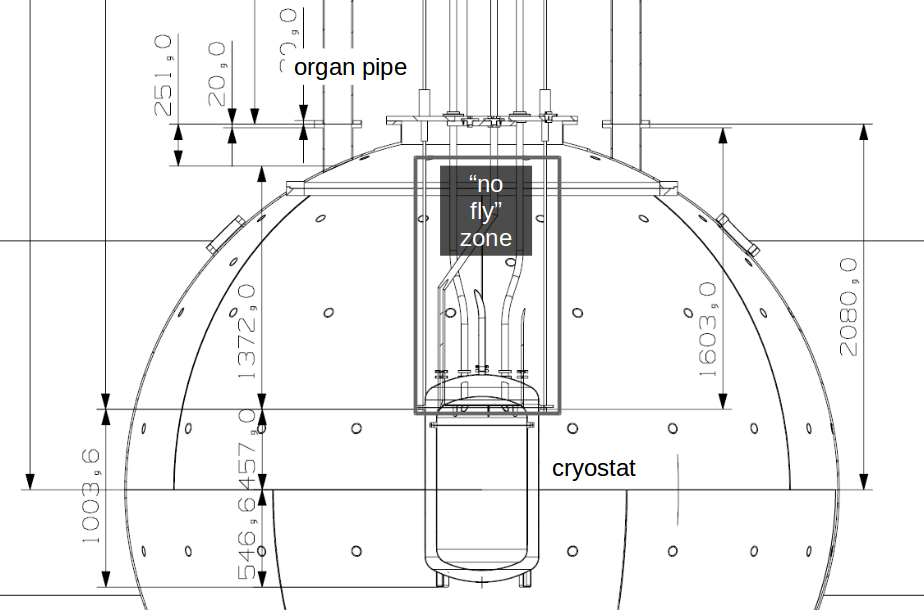
\includegraphics[scale=0.5]{Figures/NoFlyZone.png}
%  \caption{``No fly'' zone for the CALIS source arm.}
%  \label{fig:NoFlyZone}
%\end{figure} 

\subsubsection{Default configuration}
By default, deployment device has been deployed with its longest arm (62 cm), at center of TPC's active volume in vertical direction, with arm rotated in XY-plane until contact is made with cryostat. 

Other degrees of freedom could involve shorter arm lengths, while longer arm lengths would require deployment device hardware modifications. Out of four organ pipes a second one is available for source calibration. (Two organ pipes are not available due to interference with existing infrastructure: the cryogenic tower and electronic rack.) Moving CALIS to a different organ pipe requires a more substantial effort involving a partial CALIS disassembly and reinstallation on other organ pipe's gate valve.

%Finally CALIS is designed to house also a different deployment device, such as currently being planned for the neutron gun \cite{???}.